% -----------------------------------------------------------------------
% -----------------------------------------------------------------------
% -----------------------------------------------------------------------
% Einleitung
% -----------------------------------------------------------------------
% -----------------------------------------------------------------------
% -----------------------------------------------------------------------
\chapter{Einleitung}

Hier kommt eine Quellenangabe \cite{Gray1981}, \cite{Cerami2002}. Weiterhin sieht man hier einen Link auf Kapitel \ref{ch:1}.
Lorem ipsum dolor sit amet, consectetuer\footnote{Hier ist eine Fußnote!} adipiscing elit. Integer quis lectus eget purus auctor sollicitudin.
Sed tempus, leo quis nonummy iaculis, tellus justo bibendum mi, eu facilisis est sapien non eros. Ut tincidunt. Proin eleifend tristique est.
Nulla facilisi. Cras ante mauris, facilisis at, fringilla quis, venenatis ornare, libero. Nam viverra varius nibh. Suspendisse potenti.
Sed velit quam, euismod quis, sagittis eu, sodales sit amet, dui. Sed sed diam. Vivamus tincidunt quam a eros. Ut quis metus.
Lorem ipsum dolor sit amet, consectetuer adipiscing elit. Cum sociis natoque penatibus et magnis dis parturient montes, nascetur ridiculus mus.
Sed ut tortor. Vestibulum ante ipsum primis in faucibus orci luctus et ultrices posuere cubilia Curae; Curabitur vulputate nibh a tortor.
Nullam scelerisque risus nonummy urna tempor sagittis.

\noindent Hier kommt ein Listing \ref{lst:soap}.

\begin{center}
\begin{lstlisting}[caption={SOAP Anfrage an einen HalloWelt-Web-Service},label=lst:soap,language=XML,label={lst:soap}]
<?xml version='1.0' encoding='UTF-8'>
<SOAP-ENV:Envelope (*@\label{lst:soapEnv}@*)
  xmlns:SOAP-ENV="http://schemas.xmlsoap.org/soap/envelope/"
  xmlns:xsi="http://www.w3.org/2001/XMLSchema-instance"
  xmlns:xsd="http://www.w3.org/2001/XMLSchema"
  xmlns:ns1="http://localhost/wsdl/HalloWeltService.wsdl">

  <SOAP-ENV:Body>(*@\label{lst:soapBody}@*)
  	<ns1:gruss>
  		<name xsi:type="xsd:string">
  			Michael
  		</name>
  	</ns1:gruss>
  </SOAP-ENV:Body>

</SOAP-ENV:Envelope>
\end{lstlisting}
\end{center}

\begin{figure}[!ht]
  \centering
  \sourcecode{main.cpp}
  \caption{Hello World Program}\label{figure:helloworld}
\end{figure}

\begin{figure}[!ht] % see https://en.wikibooks.org/wiki/LaTeX/Floats,_Figures_and_Captions for placement parameters
  \centering
  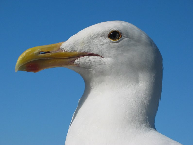
\includegraphics[width=0.5\textwidth]{images/gull.png}
  \caption{A picture of a gull. \cite{Cerami2002}}
\end{figure}
Lorem ipsum dolor sit amet, consectetuer adipiscing elit. Integer quis lectus eget purus auctor sollicitudin. Sed tempus, leo quis nonummy
iaculis, tellus justo bibendum mi, eu facilisis est sapien non eros. Ut tincidunt. Proin eleifend tristique est. Nulla facilisi. Cras ante
mauris, facilisis at, fringilla quis, venenatis ornare, libero. Nam viverra varius nibh. Suspendisse potenti. Sed velit quam, euismod quis,
sagittis eu, sodales sit amet, dui. Sed sed diam. Vivamus tincidunt quam a eros. Ut quis metus. Lorem ipsum dolor sit amet, consectetuer adipiscing elit.

\section{Motivation}
\label{ch:1}
Lorem ipsum dolor sit amet, consectetuer adipiscing elit. Integer quis lectus eget purus auctor sollicitudin. Sed tempus, leo quis nonummy
iaculis, tellus justo bibendum mi, eu facilisis est sapien non eros. Ut tincidunt. Proin eleifend tristique est. Nulla facilisi. Cras ante
mauris, facilisis at, fringilla quis, venenatis ornare, libero. Nam viverra varius nibh. Suspendisse potenti. Sed velit quam, euismod quis,
sagittis eu, sodales sit amet, dui. Sed sed diam. Vivamus tincidunt quam a eros. Ut quis metus. Lorem ipsum dolor sit amet, consectetuer adipiscing elit.

\section{Zielsetzung}
Lorem ipsum dolor sit amet, consectetuer adipiscing elit. Integer quis lectus eget purus auctor sollicitudin. Sed tempus, leo quis nonummy
iaculis, tellus justo bibendum mi, eu facilisis est sapien non eros. Ut tincidunt. Proin eleifend tristique est. Nulla facilisi. Cras ante
mauris, facilisis at, fringilla quis, venenatis ornare, libero. Nam viverra varius nibh. Suspendisse potenti. Sed velit quam, euismod quis,
sagittis eu, sodales sit amet, dui. Sed sed diam. Vivamus tincidunt quam a eros. Ut quis metus. Lorem ipsum dolor sit amet, consectetuer adipiscing elit.

\section{Eingrenzung des Themas}
\label{ch:eingrenzungThema}
Lorem ipsum dolor sit amet, consectetuer adipiscing elit. Integer quis lectus eget purus auctor sollicitudin. Sed tempus, leo quis nonummy
iaculis, tellus justo bibendum mi, eu facilisis est sapien non eros. Ut tincidunt. Proin eleifend tristique est. Nulla facilisi. Cras ante
mauris, facilisis at, fringilla quis, venenatis ornare, libero. Nam viverra varius nibh. Suspendisse potenti. Sed velit quam, euismod quis,
sagittis eu, sodales sit amet, dui. Sed sed diam. Vivamus tincidunt quam a eros. Ut quis metus. Lorem ipsum dolor sit amet, consectetuer adipiscing elit.

\section{Aufbau der Arbeit}
Lorem ipsum dolor sit amet, consectetuer adipiscing elit. Integer quis lectus eget purus auctor sollicitudin. Sed tempus, leo quis nonummy
iaculis, tellus justo bibendum mi, eu facilisis est sapien non eros. Ut tincidunt. Proin eleifend tristique est. Nulla facilisi. Cras ante
mauris, facilisis at, fringilla quis, venenatis ornare, libero. Nam viverra varius nibh. Suspendisse potenti. Sed velit quam, euismod quis,
sagittis eu, sodales sit amet, dui. Sed sed diam. Vivamus tincidunt quam a eros. Ut quis metus. Lorem ipsum dolor sit amet, consectetuer adipiscing elit.
